 \documentclass{beamer}
 \usetheme{Madrid}


%%PACKAGES

\usepackage{amsmath}
\usepackage{amsfonts}
\usepackage{amssymb}
\usepackage{amsthm}
\usepackage{graphicx}
%\usepackage{diagrams}
\usepackage{mathrsfs}
\usepackage{manfnt}
%\usepackage{pstricks}
\usepackage{tikz}
\usetikzlibrary{decorations.markings}

%%THEOREM STYLES

\theoremstyle{theorem}
\newtheorem{thm}{Theorem}
%\newtheorem{lemma}{Lemma}
\newtheorem{cor}{Corollary}
\newtheorem*{prelemma}{Lemma}
\newtheorem*{prethm}{Theorem}
\newtheorem{prop}{Proposition}
\newtheorem*{conj}{Conjecture}
\theoremstyle{definition}
\newtheorem*{defin}{Definition}
\newtheorem*{goal}{Goal}
\newtheorem*{remark}{Remark}
\newtheorem{ex}{Example}

\renewcommand{\baselinestretch}{1}

%%CUSTOM COMMANDS

\newcommand{\prob}[1]{\subsection*{#1}}
\newcommand{\subprob}[1]{\subsubsection*{#1}}


\newcommand{\R}{\ensuremath{\mathbb R}}
\newcommand{\A}{\ensuremath{\mathbb A}}
\newcommand{\Z}{\ensuremath{\mathbb Z}}
\newcommand{\C}{\ensuremath{\mathbb C}}
\newcommand{\Q}{\ensuremath{\mathbb Q}}
\newcommand{\T}{\ensuremath{\mathbb T}}
\renewcommand{\H}{\ensuremath{\mathbb H}}
\newcommand{\CP}{\ensuremath{\mathbf{CP}}}
\newcommand{\RP}{\ensuremath{\mathbf{RP}}}
\renewcommand{\P}{\ensuremath{\mathbf P}}
\newcommand{\eset}{\emptyset}

\newcommand{\isom}{\cong}
\renewcommand{\implies}{\Rightarrow}
\renewcommand{\iff}{\Leftrightarrow}

\renewcommand{\O}{\ensuremath{\mathcal{O}}}
\newcommand{\F}{\ensuremath{\mathcal F}}
\newcommand{\G}{\ensuremath{\mathcal{G}}}
\newcommand{\I}{\ensuremath{\mathscr{I}}}
\newcommand{\E}{\ensuremath{\mathcal{E}}}
\newcommand{\M}{\ensuremath{\mathcal{M}}}
\newcommand{\K}{\ensuremath{\mathcal{K}}}
\newcommand{\N}{\ensuremath{\mathbf{N}}}
\newcommand{\U}{\ensuremath{\mathfrak U}}

\newcommand{\cech}{\check{\text{C}}\text{ech}}

\renewcommand{\a}{\ensuremath{\mathfrak a}}
\newcommand{\m}{\ensuremath{\mathfrak m}}
\newcommand{\p}{\ensuremath{\mathfrak p}}
\newcommand{\q}{\ensuremath{\mathfrak q}}
\newcommand{\e}{\ensuremath{\epsilon}}

\newcommand{\vphi}{\varphi}


\newcommand{\Div}{\ensuremath{\operatorname{Div}}}
\newcommand{\spec}{\ensuremath{\operatorname{Spec}}}
\newcommand{\rank}{\ensuremath{\operatorname{rank}}}
\newcommand{\injrad}{\ensuremath{\operatorname{inj}}}
\newcommand{\vol}{\ensuremath{\operatorname{vol}}}
\newcommand{\End}{\ensuremath{\operatorname{End}}}
\newcommand{\iso}{\ensuremath{\operatorname{Isom}}}
\newcommand{\proj}{\ensuremath{\operatorname{Proj}}}
\newcommand{\hgt}{\operatorname{ht}}
\newcommand{\im}{\operatorname{Im}}
\renewcommand{\hom}{\operatorname{Hom}}
\newcommand{\adj}{\operatorname{Adj}}
\renewcommand{\-}{\ensuremath{^{-1}}}
\renewcommand{\>}{\ensuremath{\rightarrow}}
\newcommand{\map}{\ensuremath{\mapsto}}
\newcommand{\id}{\ensuremath{\mathbf{Id}}}
\newcommand{\pr}{^{\prime}}
\newcommand{\rad}{\operatorname{Rad}}
\newcommand{\ann}{\operatorname{Ann}}
\newcommand{\ass}{\operatorname{Ass}}
\newcommand{\supp}{\operatorname{Supp}}
\newcommand{\coker}{\operatorname{coker}}
\newcommand{\del}{\partial}


\renewcommand{\(}{\langle}
\renewcommand{\)}{\rangle}
\newcommand{\inject}{\hookrightarrow}
\newcommand{\surject}{\twoheadrightarrow}
\newcommand{\Aut}{\text{Aut}\,}
\newcommand{\Out}{\text{Out}}
%\newcommand{\End}{\text{End}\,}
\newcommand{\ad}{\text{ad}\,}
\newcommand{\Ad}{\text{Ad}\,}

\newcommand{\invlim}{\mathop{\varprojlim}\limits}
\newcommand{\directlim}{\mathop{\varinjlim}\limits}

\newcommand{\surj}{\twoheadrightarrow}
\newcommand{\inj}{\hookrightarrow}

\renewcommand{\part}[2]{\frac{\del{#1}}{\del{#2}}}

%MARGINS

%\usepackage[left=1in,top=1in,right=1in,bottom=1in]{geometry}

\AtBeginSection[] {
\begin{frame}<beamer>
   \frametitle{Sections}
   \tableofcontents[currentsection]
\end{frame}}

\title{PhD Thesis Defense}
\subtitle{Some Hyperbolic $Out(F_N)$-Graphs and\\ Non-Unique Ergodicity of\\ Very Small $F_N$-trees}
\author{Brian Mann}
\institute{University of Utah}
\date{February 26, 2014}

\begin{document}

\begin{frame}
\titlepage
\end{frame}



\section{Preliminaries}

\begin{frame}
You can get all these slides on \url{http://www.github.com/brianmannmath/thesis_defense}
\end{frame}


\begin{frame}
\frametitle{Goal}
Fix $N \geq 3$. Let $F_N$ be the free group of rank $N$. We are trying to study $Out(F_N) = Aut(F_N)/Inn(F_N)$ by finding well-behaved actions on interesting spaces.

\vspace{1cm}

\pause

Today, an \emph{interesting space} is a \emph{hyperbolic metric space} and \emph{well-behaved} means something like \emph{nontrivial, isometric}.

\vspace{1cm} 
\pause

Motivated by results of Masur and Minksy (the curve complex is hyperbolic \cite{MasurMinsky}), Bestvina and Feighn (the free factor complex is hyperbolic \cite{BF11}), and Handel and Mosher (the free splitting graph is hyperbolic \cite{HandelMosher}) as well as many others.
\end{frame}



\begin{frame}
\frametitle{The Cyclic Splitting Graph}
What's an example of such a space? Consider the simplicial graph $FZ_N$ defined as follows:
\pause
\begin{itemize}
\item The vertices of $FZ_N$ are one-edge splittings of $F_N$ (up to conjugacy) with $\Z$ or trivial edge group.
\pause
\item There is an edge between splittings $T$ and $S$ if there exists a two-edge splitting $R$ refining both $T$ and $S$.
\end{itemize}

$FZ_N$ is the \emph{cyclic splitting graph}. It has a natural $Out(F_N)$-action.
\end{frame}

\begin{frame}
\frametitle{Example}
The splittings of $F_5$
\begin{center}
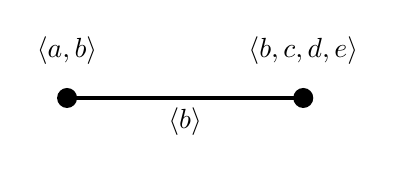
\begin{tikzpicture}[scale = 3, very thick]
\filldraw [black] (0,0) circle (1pt)
			(1,0) circle (1pt);
\draw (0,0) -- (1,0) node[scale = 1] at (0,.2) {$\(a,b\)$} node[scale = 1] at (.5,-.1) {$\(b\)$ }node[scale = 1] at (1,.2) {$\(b,c,d,e\)$};
\end{tikzpicture}
\end{center}
\pause
and
\begin{center}
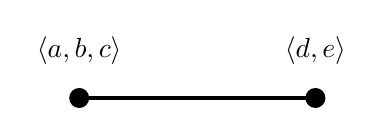
\begin{tikzpicture}[scale = 3, very thick]
\filldraw [black] (0,0) circle (1pt)
			(1,0) circle (1pt);
\draw (0,0) -- (1,0) node[scale = 1] at (0,.2) {$\(a,b,c\)$} node[scale = 1] at (1,.2) {$\(d,e\)$};
\end{tikzpicture}
\end{center}
\pause
are commonly refined by
\begin{center}
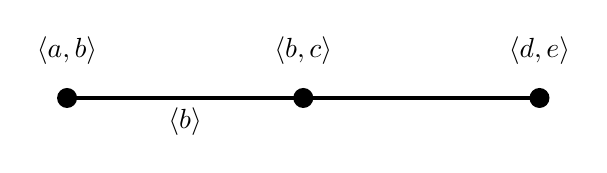
\begin{tikzpicture}[scale = 3, very thick]
\filldraw [black] (0,0) circle (1pt)
			(1,0) circle (1pt)
			(2,0) circle (1pt);
\draw (0,0) -- (1,0) -- (2,0) node[scale = 1] at (0,.2) {$\(a,b\)$} node[scale = 1] at (.5,-.1) {$\(b\)$ }node[scale = 1] at (1,.2) {$\(b,c\)$} node at (2,.2) {$\(d,e\)$};
\end{tikzpicture}
\end{center}
\end{frame}

\begin{frame}
\frametitle{First Main Result}
\begin{thm}[M \cite{Mann13}]
The cyclic splitting graph with the simplicial metric (every edge is length 1) is $\delta$-hyperbolic. 
\end{thm}
\end{frame}

\section{A sketch of the proof of the first main theorem}

\begin{frame}
\frametitle{The main tool}
Kapovich and Rafi proved the following, using Bowditch's \cite{Bowditch} \emph{thin-triangles} condition for hyperbolicity.
\pause
\begin{thm}[Kapovich-Rafi \cite{KapovichRafi}]
Suppose $X$ and $Y$ are connected graphs, $X$ is hyperbolic, and $f : X \> Y$ is Lipschitz. Suppose there is $S \subseteq V(X)$ such that
\begin{enumerate}
\item $f(S) = V(Y)$ 
\item $S$ is $D$-dense in $V(X)$ for some $D \geq 0$. 
\item There is an $M > 0$ such that if $x,y \in S$ with $d(f(x),f(y)) \leq 1$ then $diam(f[x,y]) \leq M$. 
\end{enumerate}
Then $Y$ is hyperbolic.
\end{thm}
\end{frame}

\begin{frame}
\frametitle{How do we use it?}
By Handel-Mosher \cite{HandelMosher} we know that the free splitting graph $FS_N$ is hyperbolic.
\pause 
\vspace{1cm}

We use a quasi-isometric model of $FZ_N$ and a natural, $Out(F_N)$-equivariant map $FS_N \> FZ_N$ which clearly satisfies the first two conditions of the above theorem.
\end{frame}

\begin{frame}
\frametitle{What about the third condition?}
Essentially, it boils down to proving the following claim: 
\pause
\vspace{1cm}

If $R$ and $R\pr$ are marked roses (free splittings of $F_N$ with 1 vertex and $N$ edges) whose images in $FZ_N$ are close, then the Handel-Mosher folding path from $R$ to $R\pr$ stays uniformly bounded in $FZ_N$. 
\end{frame}

\section{More cyclic splitting complex}

\begin{frame}
\frametitle{It really is something new!}
Ok, the title is a little bold, but...
\pause
\begin{prop}
$FS_N$ and $FZ_N$ are not $Out(F_N)$-equivariantly quasi-isometric. 
\end{prop}
\pause
\begin{proof}
\begin{center}
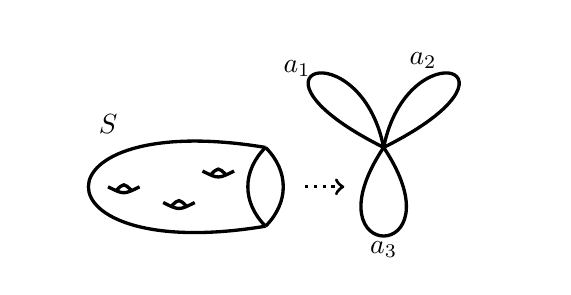
\begin{tikzpicture}[scale = 1,very thick]
	%draws the outline of the surface
	\draw node[scale = 1] at (-2,1.3) {$S$};
	\draw (0,0) .. controls (-3,-.5) and (-3,1.5) .. (0,1);
	\draw (0,0) .. controls (.3,.3) and (.3,.7) .. (0,1);
	\draw (0,0) .. controls (-.3,.3) and (-.3,.7) .. (0,1);
	
	%draw the first genus
	\draw (-2,.5) .. controls ++(.2,-.1) .. ++(.4,0) ;
	\draw (-1.9,.45) .. controls ++(.1,.1) .. ++(.2,0);
	
	%draw the second genus
	\draw (-1.3,.3) .. controls ++(.2,-.1) .. ++(.4,0) ;
	\draw (-1.2,.25) .. controls ++(.1,.1) .. ++(.2,0);
	
	%draw the third genus
	\draw (-.8,.7) .. controls ++(.2,-.1) .. ++(.4,0) ;
	\draw (-.7,.65) .. controls ++(.1,.1) .. ++(.2,0);
	
	%attaching map arrow
	\draw[->,dotted] (.5,.5) -- (1,.5); 
	
	%the rose
	\draw (1.5,1) .. controls ++(-1,-1.5) and ++(1,-1.5) .. (1.5,1) node[scale = 1] at (1.5,-.3) {$a_3$};
	\draw (1.5,1) .. controls ++(.3,1.5) and ++(2,1) .. (1.5,1) node[scale = 1] at (.4,2) {$a_1$};
	\draw (1.5,1) .. controls ++(-.3,1.5) and ++(-2,1) .. (1.5,1) node[scale = 1] at (2,2.1) {$a_2$};
	
		
\end{tikzpicture}
\end{center}
(Don't worry, I'll explain on the board.)
\end{proof}
\end{frame}

\section{More results}

\begin{frame}
Define a graph $I_N$ whose vertices are one-edge very small $F_N$-trees, and where two trees $T$ and $T\pr$ are connect by and edge if there exists a measured current $\mu$ such that $\(T,\mu\) = 0 = \(T\pr,\mu\)$. 
\pause
\begin{thm}[M 2014]
$I_N$ is hyperbolic, and furthermore the action of $Out(F_N)$ on $I_N$ satisfies Bestvina and Fujiwara's Weak Proper Discontinuity condition \cite{BF02}.
\end{thm}
\end{frame}

\begin{frame}
\frametitle{Nonuniquely ergodic $F_N$-trees}
An arational $F_N$-tree $T$ in $\del CV_N$ is \emph{nonuniquely ergodic} if there exist distinct non-homothetic length measures on $T$.
\pause
\begin{thm}[M-Reynolds \cite{MR13} 2013]
Given two curves (a certain type of one-edge very small $\Z$-splitting of $F_N$) with neighborhoods $U$ and $U\pr$ in $\del CV_N$, there is a $1$-simplex of nonuniquely ergodic, arational, nongeometric trees with one endpoint in each of $U, U\pr$.  
\end{thm}
\end{frame}

\begin{frame}
\frametitle{Acknowledgements}

I'd like to thank 
\begin{itemize}
\item Mladen for agreeing to be my advisor, answering my dumb questions, being exceptionally patient, and not being too annoyed when I forgot to double check when we were supposed to meet.

\item Patrick for putting up with the questions I thought were too dumb to ask to Mladen, for teaching me about being a co-author, and for introducing me to the Marseille $Out(F_N)$ people.

\item Ric for talking with me about math in pubs, giving me places to stay in and showing me around the UK, and not getting too annoyed when I was trying to avoid working out details.

\item Ken Bromberg, Ilya Kapovich, Kasra Rafi, Juan Souto, and Kevin Wortman for talking with me about math (and being a mathematician) during my undergrad and graduate careers.    

\item All my fellow grad students who made my time here a lot of fun.
\end{itemize}
\end{frame}

\bibliographystyle{plain}
\bibliography{Refs,indecompREF}
\end{document}
















\end{document}

